% !TEX TS-program = XeLaTeX
% use the following command:
% all document files must be coded in UTF-8
\documentclass[spanish]{textolivre}
% build HTML with: make4ht -e build.lua -c textolivre.cfg -x -u article "fn-in,svg,pic-align"

\journalname{Texto Livre}
\thevolume{15}
%\thenumber{1} % old template
\theyear{2022}
\receiveddate{\DTMdisplaydate{2021}{11}{15}{-1}} % YYYY MM DD
\accepteddate{\DTMdisplaydate{2022}{1}{4}{-1}}
\publisheddate{\today}
\corrauthor{Ricardo-Adán Salas-Rueda}
\articledoi{10.35699/1983-3652.2022.37074}
%\articleid{NNNN} % if the article ID is not the last 5 numbers of its DOI, provide it using \articleid{} commmand
\runningauthor{Salas-Rueda et al.} 
%\editorname{Leonardo Araújo} % old template
\sectioneditorname{Hugo Heredia Ponce}
\layouteditorname{Anna Izabella Pereira}

\title{Percepción de los profesores sobre los juegos web y dispositivos móviles en el nivel educativo superior durante la pandemia COVID-19}
\othertitle{Percepção dos professores sobre jogos da web e dispositivos móveis no nível educacional superior durante a pandemia de COVID-19}
\othertitle{Teachers' perception of web games and mobile devices at the higher educational level during the COVID-19 pandemic}
% if there is a third language title, add here:
%\othertitle{Artikelvorlage zur Einreichung beim Texto Livre Journal}

\author[1]{Ricardo-Adán Salas-Rueda \orcid{0000-0002-4188-4610} \thanks{Email: \url{ricardo.salas@icat.unam.mx}}}
\author[1]{Jesús Ramírez-Ortega \orcid{0000-0002-4538-9203} \thanks{Email: \url{jesus.ramirez@icat.unam.mx}}}
\author[1]{Ana-Libia Eslava-Cervantes \orcid{0000-0002-7420-3412} \thanks{Email: \url{libia.eslava@icat.unam.mx}}}
\author[1]{Ricardo Castañeda-Martínez \orcid{0000-0002-2225-7136} \thanks{Email: \url{ricardo.castaneda@icat.unam.mx}}}
\author[1]{Gustavo De-La-Cruz-Martínez \orcid{0000-0002-4446-7396} \thanks{Email: \url{gustavo.delacruz@icat.unam.mx}}}

\affil[1]{Universidad Nacional Autónoma de México, Instituto de Ciencias Aplicadas y Tecnología, Ciudad de México, México.}

\addbibresource{article.bib}
% use biber instead of bibtex
% $ biber article

% used to create dummy text for the template file
\definecolor{dark-gray}{gray}{0.35} % color used to display dummy texts
\usepackage{lipsum}
\SetLipsumParListSurrounders{\colorlet{oldcolor}{.}\color{dark-gray}}{\color{oldcolor}}

% used here only to provide the XeLaTeX and BibTeX logos
\usepackage{hologo}

% if you use multirows in a table, include the multirow package
\usepackage{multirow}

% provides sidewaysfigure environment
\usepackage{rotating}

% CUSTOM EPIGRAPH - BEGIN 
%%% https://tex.stackexchange.com/questions/193178/specific-epigraph-style
\usepackage{epigraph}
\renewcommand\textflush{flushright}
\makeatletter
\newlength\epitextskip
\pretocmd{\@epitext}{\em}{}{}
\apptocmd{\@epitext}{\em}{}{}
\patchcmd{\epigraph}{\@epitext{#1}\\}{\@epitext{#1}\\[\epitextskip]}{}{}
\makeatother
\setlength\epigraphrule{0pt}
\setlength\epitextskip{0.5ex}
\setlength\epigraphwidth{.7\textwidth}
% CUSTOM EPIGRAPH - END

% LANGUAGE - BEGIN
% ARABIC
% for languages that use special fonts, you must provide the typeface that will be used
% \setotherlanguage{arabic}
% \newfontfamily\arabicfont[Script=Arabic]{Amiri}
% \newfontfamily\arabicfontsf[Script=Arabic]{Amiri}
% \newfontfamily\arabicfonttt[Script=Arabic]{Amiri}
%
% in the article, to add arabic text use: \textlang{arabic}{ ... }
%
% RUSSIAN
% for russian text we also need to define fonts with support for Cyrillic script
% \usepackage{fontspec}
% \setotherlanguage{russian}
% \newfontfamily\cyrillicfont{Times New Roman}
% \newfontfamily\cyrillicfontsf{Times New Roman}[Script=Cyrillic]
% \newfontfamily\cyrillicfonttt{Times New Roman}[Script=Cyrillic]
%
% in the text use \begin{russian} ... \end{russian}
% LANGUAGE - END

% EMOJIS - BEGIN
% to use emoticons in your manuscript
% https://stackoverflow.com/questions/190145/how-to-insert-emoticons-in-latex/57076064
% using font Symbola, which has full support
% the font may be downloaded at:
% https://dn-works.com/ufas/
% add to preamble:
% \newfontfamily\Symbola{Symbola}
% in the text use:
% {\Symbola }
% EMOJIS - END

% LABEL REFERENCE TO DESCRIPTIVE LIST - BEGIN
% reference itens in a descriptive list using their labels instead of numbers
% insert the code below in the preambule:
%\makeatletter
%\let\orgdescriptionlabel\descriptionlabel
%\renewcommand*{\descriptionlabel}[1]{%
%  \let\orglabel\label
%  \let\label\@gobble
%  \phantomsection
%  \edef\@currentlabel{#1\unskip}%
%  \let\label\orglabel
%  \orgdescriptionlabel{#1}%
%}
%\makeatother
%
% in your document, use as illustraded here:
%\begin{description}
%  \item[first\label{itm1}] this is only an example;
%  % ...  add more items
%\end{description}
% LABEL REFERENCE TO DESCRIPTIVE LIST - END


% add line numbers for submission
%\usepackage{lineno}
%\linenumbers

\begin{document}
\maketitle

\begin{polyabstract}
\begin{abstract}
El virus SARS-CoV-2 ha provocado que las universidades busquen nuevas alternativas tecnológicas con el propósito de mejorar la enseñanza y el aprendizaje bajo la modalidad a distancia. Esta investigación cuantitativa y cualitativa analiza la percepción de los educadores sobre los juegos web y dispositivos móviles durante la pandemia COVID-19 considerando la técnica aprendizaje automático y la técnica árbol de decisión (ciencia de datos). Los participantes son 60 docentes de educación superior que impartieron cursos en la Universidad Nacional Autónoma de México en el año 2021 y tomaron el Diplomado “Innovación en la Docencia Universitaria 2021”. La técnica aprendizaje automático indica que el uso de los juegos web y dispositivos móviles influyen positivamente la labor docente y participación de los estudiantes durante el proceso de enseñanza-aprendizaje. Además, la ciencia de datos establece 4 modelos predictivos sobre estas herramientas tecnológicas a través de la técnica árbol de decisión. Por último, los juegos web y dispositivos móviles permiten la creación de nuevos espacios virtuales que favorecen la enseñanza bajo la modalidad a distancia y facilitan el aprendizaje desde cualquier lugar.

\keywords{Educadores \sep Dispositivos móviles \sep TIC \sep Enseñanza \sep Ciencia de datos}
\end{abstract}

\begin{portuguese}
\begin{abstract}
O vírus SARS-CoV-2 tem feito com que as universidades busquem novas alternativas tecnológicas para aprimorar o ensino e a aprendizagem na modalidade a distância. Esta pesquisa quantitativa e qualitativa analisa a percepção de educadores sobre jogos para \textit{web} e dispositivos móveis durante a pandemia de COVID-19, considerando a técnica de aprendizado de máquina e a técnica de árvore de decisão (ciência de dados). Os participantes são 60 professores de educação superior que ministraram cursos na Universidade Nacional Autônoma do México em 2021 e obtiveram o diploma “Inovação no Ensino Universitário 2021”. A técnica de aprendizado de máquina indica que o uso de \textit{web games} e dispositivos móveis influenciam positivamente o trabalho docente e a participação dos alunos durante o processo ensino-aprendizagem. Além disso, a \textit{data science} estabelece quatro modelos preditivos sobre essas ferramentas tecnológicas por meio da técnica de árvore de decisão. Por fim, os \textit{web games} e dispositivos móveis permitem a criação de novos espaços virtuais que favorecem o ensino a distância e facilitam o aprendizado de qualquer lugar.

\keywords{Educadores \sep Dispositivos móveis \sep TIC \sep Ensino \sep Ciência de dados}
\end{abstract}
\end{portuguese}

\begin{english}
\begin{abstract}
The SARS-CoV-2 virus has caused universities to search for new technological alternatives in order to improve the teaching and learning in distance modality. This quantitative and qualitative research analyzes the perception of educators about web games and mobile devices during the COVID-19 pandemic considering the machine learning technique and decision tree technique (data science). The participants are 60 teachers of higher education who taught courses at the National Autonomous University of Mexico in 2021 and took the “Innovation in University Teaching 2021” Diploma. The machine learning technique indicates that the use of web games and mobile devices positively influences the teaching work and participation of the students during the teaching-learning process. In addition, data science establishes 4 predictive models about these technological tools through the decision tree technique. Finally, web games and mobile devices allow the creation of new virtual spaces that favor distance teaching and facilitate learning from anywhere.

\keywords{Educators \sep Mobile devices \sep ICT \sep Teaching \sep Data science}
\end{abstract}
\end{english}
% if there is another abstract, insert it here using the same scheme
\end{polyabstract}

\section{Introdução}\label{sec-intro}
Actualmente, el virus SARS-CoV-2 está provocando que todos los niveles educativos cambien la organización y planeación de los cursos a través de la incorporación de las Tecnologías de la Información y Comunicación (TIC) en las actividades escolares \cite{maphosa2021, maggio2020, ramirez-montoya2020}. En particular, los docentes utilizan las herramientas tecnológicas para impartir las asignaturas desde cualquier lugar bajo la modalidad a distancia \cite{manrique-losada2020, saribas2021}.

Los avances tecnológicos como los dispositivos móviles abren la posibilidad de organizar y realizar creativas actividades escolares durante, después y antes de las clases \cite{gezgin2018, park2020}. De hecho, los teléfonos inteligentes adquieren un rol principal durante la ejecución del proceso de enseñanza-aprendizaje debido a que los estudiantes buscan, comparten, consultan y usan la información en cualquier momento \cite{padmo2019, sumuer2021}. Los beneficios relacionados con el uso de los teléfonos inteligentes, las tabletas y las computadoras portátiles en el campo educativo son la flexibilidad de tiempo y espacio \cite{park2020}.

Del mismo modo, los juegos web están cambiando las funciones y las responsabilidades de los docentes y estudiantes \cite{felszeghy2019, ismail2019}. En particular, Kahoot es un juego web que facilita el aprendizaje y la enseñanza en las modalidades presencial y a distancia \cite{licorish2018, ismail2019}. La incorporación de los juegos web en las actividades escolares promueve, fomenta y desarrolla las habilidades y el rol activo de los alumnos \cite{donald2017, smith2020}.

Debido a la pandemia COVID-19, las universidades y los maestros están actualizando e innovando las actividades escolares con el apoyo de las herramientas tecnológicas bajo la modalidad a distancia con el propósito de satisfacer las demandas y necesidades de los estudiantes. El Diplomado “Innovación en la Docencia Universitaria 2021” de la Universidad Nacional Autónoma de México busca capacitar a los docentes en los temas relacionados con las estrategias educativas y el uso de las TIC. De hecho, estos educadores buscan, seleccionan y utilizan los avances tecnológicos como los juegos web y dispositivos móviles para mejorar la realización del proceso de enseñanza-aprendizaje bajo la modalidad a distancia y construir nuevos espacios virtuales educativos. 

Por consiguiente, el objetivo general de esta investigación mixta es analizar la percepción de los educadores sobre los juegos web y dispositivos móviles en el nivel educativo superior durante la pandemia COVID-19 considerando la técnica aprendizaje automático y la técnica árbol de decisión (ciencia de datos).

Las preguntas de este estudio cuantitativo y cualitativo son:
\begin{itemize}
    \item ¿Cuál es la percepción de los maestros sobre los juegos web y dispositivos móviles en el nivel educativo superior considerando la técnica aprendizaje automático? 
    \item ¿Cuáles son los modelos predictivos sobre los juegos web y dispositivos móviles  considerando el perfil de los maestros (técnica árbol de decisión)? \item ¿Cuál es la percepción de los maestros sobre los juegos web y dispositivos móviles en el nivel educativo superior durante la pandemia COVID-19? 
\end{itemize}

\section{Revisión de la literatura}
Hoy en día, las universidades, preparatorias, secundarias y primarias utilizan las TIC para innovar el proceso de enseñanza-aprendizaje bajo las modalidades presencial y mixta \cite{felszeghy2019, karatas2021}. En particular, los avances tecnológicos como los juegos web y dispositivos móviles permiten la creación y organización de espacios educativos que promueven y fomentan el rol activo y la participación de los estudiantes \cite{ismail2019, saribas2021}. 

\subsection{Dispositivos móviles}
De acuerdo con \textcite{maphosa2021}, las funciones de los educadores relacionadas con la organización y ejecución de las actividades escolares han cambiado debido al surgimiento del COVID-19. Por ejemplo, los docentes utilizan los dispositivos móviles (p. ej., teléfonos inteligentes, computadoras portátiles y tabletas) para mejorar las condiciones de aprendizaje en diversos países como Indonesia \cite{padmo2019}, Turquía \cite{gezgin2018, sumuer2021}, Estados Unidos \cite{park2020}, Malasia \cite{arumugam2021} y China \cite{li2019}.

En Indonesia, la incorporación de los teléfonos inteligentes en la Universidad de Terbuka facilitó el proceso de enseñanza-aprendizaje en la modalidad educación a distancia debido a que los estudiantes consultaron la información de los cursos en cualquier momento y realizaron las actividades escolares desde cualquier lugar \cite{padmo2019}. De acuerdo con \textcite{gezgin2018}, los alumnos de la Ingeniería en Computación incrementaron sus calificaciones y satisfacción a través del uso de los dispositivos móviles fuera y dentro del aula.

Del mismo modo, los estudiantes de la Licenciatura en Enfermería emplearon los dispositivos móviles para revisar los recursos multimedia, consultar la información y realizar los exámenes sobre los temas de la conducta clínica \cite{li2019}. Incluso, el uso de aplicaciones en los teléfonos inteligentes incrementó la motivación y satisfacción de estos alumnos durante el curso de medicina \cite{li2019}.

En Europa, los estudiantes utilizan las herramientas de realidad virtual en los dispositivos móviles para incrementar su rendimiento académico, facilitar la asimilación del conocimiento y desarrollar sus habilidades en cualquier momento \cite{al_farsi2021}. En la Universidad Católica de Manizales, las aplicaciones móviles de realidad aumentada mejoraron el rol activo de los estudiantes y facilitaron el aprendizaje sobre las superficies en el curso de Ingeniería \cite{carmona-ramirez2021}.

De acuerdo con \textcite{arumugam2021}, los dispositivos móviles y las aplicaciones tecnológicas están cambiando la organización y la realización de las actividades escolares en los cursos del Idioma Extranjero.  Por ejemplo, la aplicación móvil llamada JuJu facilitó el proceso de aprendizaje sobre el idioma Inglés y desarrolló las habilidades gramaticales de los estudiantes en una universidad de Malasia \cite{arumugam2021}.

En el campo de las matemáticas, la incorporación de la aplicación GeoGebra y el uso de los dispositivos móviles facilitaron el aprendizaje y desarrollaron las habilidades de los estudiantes dentro y fuera del aula \cite{samura2021}. Asimismo, los beneficios sobre el empleo de WhatsApp en los teléfonos inteligentes son la comunicación entre los participantes del proceso educativo desde cualquier lugar y el desarrollo de las habilidades \cite{morsidi2021}.

En Turquía, los estudiantes de preparatoria incrementaron su rendimiento académico por medio del uso de los teléfonos inteligentes \cite{sumuer2021}. Del mismo modo, la incorporación de las tabletas en el curso Lengua Extranjera desarrolló las habilidades de comunicación, verbales y gramaticales \cite{park2020}.

Por último, los maestros emplean los dispositivos móviles para innovar y actualizar las actividades de las asignaturas y fomentar el rol activo de los alumnos \cite{park2020, sumuer2021}. De hecho, el teléfono inteligente facilita el aprendizaje desde la casa, el aula, el laboratorio y el trabajo \cite{li2019, padmo2019}.

\subsection{Juegos web}\label{sec-formato}
Debido al COVID-19, los educadores han modificado sus prácticas y actividades con el apoyo de las TIC \cite{bawaaneh2021, saribas2021}. Por ejemplo, el uso de los juegos web como herramienta de apoyo mejoró las condiciones de enseñanza  y facilitó el aprendizaje sobre la medicina \cite{donald2017, smith2020}, la ingeniería \cite{de_la_pena_esteban2020}, los sistemas industriales \cite{de_la_pena_esteban2020}, el idioma inglés \cite{licorish2018} y la estadística \cite{salas-rueda2020}.

En la Universidad Abertay, los estudiantes de Medicina mejoraron su rendimiento académico sobre el entrenamiento clínico por medio de un juego web \cite{donald2017}. Del mismo modo, los alumnos de Medicina en Canadá utilizaron un juego web sobre las enfermedades infecciosas para asimilar el conocimiento desde cualquier lugar, desarrollar sus habilidades en cualquier momento e incrementar su motivación durante el proceso educativo \cite{smith2020}.

\textcite{de_la_pena_esteban2020} diseñaron y construyeron un juego para aprender las técnicas de optimización en los sistemas industriales. Los beneficios de este juego web son el desarrollo de las habilidades y el incremento del rendimiento de los alumnos \cite{de_la_pena_esteban2020}.

Asimismo, \textcite{salas-rueda2020} construyeron un juego web sobre la estadística descriptiva llamado Web Game On Descriptive Statistics (WGODS) con la finalidad de desarrollar las habilidades matemáticas de los estudiantes y comprender los temas sobre la frecuencia.

Por último, los avances tecnológicos como los juegos web permiten que los  alumnos participen activamente durante, antes y después de las sesiones presenciales \cite{donald2017, felszeghy2019, licorish2018}. En particular, los juegos web permiten la creación y planeación de espacios virtuales educativos donde el estudiante es el eje principal del proceso de aprendizaje \cite{de_la_pena_esteban2020, ypsilanti2014}.

\subsection{Ciencia de datos}
La ciencia de datos permite la identificación, evaluación y clasificación de la información \cite{hilbert2021, lezhnina2021}. En particular, el aprendizaje automático conocido en el idioma inglés como machine learning utiliza los algoritmos de regresión lineal, regresión logística, árbol de decisión, bosques aleatorios, red neuronal y Bayes Naive para resolver los problemas \cite{chadaga2021, radwan2017}.

La técnica de aprendizaje automático es utilizada para identificar las relaciones existentes entre las variables independiente y dependiente \cite{chadaga2021, lezhnina2021, radwan2017}. Por otro lado, la técnica árbol de decisión clasifica la información con la finalidad de identificar y predecir los eventos de los fenómenos \cite{chadaga2021}.

En el campo de la medicina, el aprendizaje automático tiene un papel fundamental durante el estudio de la pandemia COVID-19 debido a que esta técnica de ciencia de datos permite diagnosticar las enfermedades y predecir las condiciones de propagación por medio de las regresiones \cite{chadaga2021}. Del mismo modo, \textcite{hilbert2021} utilizó el aprendizaje automático para identificar las condiciones que influyen durante la aplicación de tratamientos en las clínicas.

En el campo de la educación, el aprendizaje automático permitió identificar las habilidades de los niños con autismo \cite{radwan2017}. Asimismo, \textcite{lezhnina2021} utilizaron la técnica de bosques aleatorios para identificar las condiciones que afectan la actitud de los estudiantes durante el uso de las herramientas tecnológicas \cite{lezhnina2021}. Incluso, \textcite{salas-rueda2021} utilizó la técnica de aprendizaje automático para identificar el efecto de las TIC y el Aula invertida en el curso Matemáticas Financieras y la técnica árbol de decisión para determinar los modelos predictivos a través del sexo y la edad de los alumnos.

Por último, el aprendizaje automático permite conocer las relaciones entre las variables de investigación, identificar las condiciones predictivas de los eventos y clasificar la información con la finalidad de descubrir nuevo conocimiento que facilite el entendimiento de los fenómenos que nos rodean \cite{chadaga2021, hilbert2021, lezhnina2021}.

\section{Metodología}
Los objetivos particulares de esta investigación cuantitativa y cualitativa son (1) analizar la percepción de los maestros sobre el uso de los juegos web y dispositivos móviles en la labor docente y participación de los estudiantes durante el proceso de enseñanza-aprendizaje por medio de la técnica aprendizaje automático (2) identificar los modelos predictivos sobre los juegos web y dispositivos móviles considerando el perfil de los docentes a través de la ciencia de datos (técnica árbol de decisión) y (3) analizar la percepción de los docentes sobre el uso de los juegos web y dispositivos móviles en el nivel educativo superior durante la pandemia COVID-19.

\subsection{Participantes}
Los participantes son 60 docentes (17 hombres y 43 mujeres) de educación superior que impartieron cursos en la Universidad Nacional Autónoma de México en el año 2021. Estos profesores poseen el grado de Doctorado (n = 12, 20.00\%), Maestría (n = 33, 55.00\%) y Licenciatura (n = 15, 25.00\%). La edad promedio es 44.55 años. Asimismo, estos docentes cursaron el Diplomado “Innovación en la Docencia Universitaria 2021” (Ver \Cref{fig1}). Esta investigación utilizó el muestreo no probabilístico.

\begin{figure}[htbp]
 \centering
 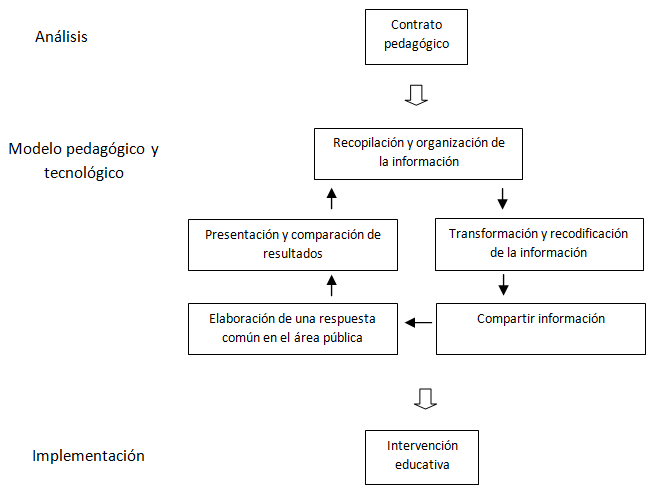
\includegraphics[width=0.6\textwidth]{37074-pag1.png}
 \caption{Diplomado “Innovación en la Docencia Universitaria 2021”.}
 \label{fig1}
 \source{Elaboración propia.}
\end{figure}

\subsection{Procedimiento}
La pandemia COVID-19 ha provocado que los docentes busquen nuevas opciones tecnológicas que faciliten el proceso de enseñanza-aprendizaje bajo la modalidad a distancia. La Figura 2 muestra el modelo utilizado en este estudio. Las variables independientes son los juegos web y dispositivos móviles. Asimismo, las variables dependientes son la labor docente y participación de los estudiantes. La técnica aprendizaje automático permite identificar las relaciones entre estas variables por medio de la regresión lineal y la técnica árbol de decisión permite determinar los modelos predictivos por medio del perfil del docente.

\begin{figure}[htbp]
 \centering
 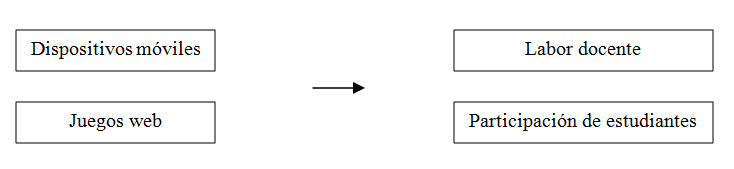
\includegraphics[width=0.7\textwidth]{37074-pag2.png}
 \caption{Modelo sobre el uso de los juegos web y dispositivos móviles.}
 \label{fig2}
 \source{Elaboración propia.}
\end{figure}

Diversos autores \cite[p. ej.]{gezgin2018, li2019, padmo2019, sumuer2021} mencionan que los dispositivos móviles como las tabletas y los celulares inteligentes permiten innovar las actividades escolares. Por lo tanto, las hipótesis sobre esta herramienta tecnológica son:

\begin{itemize}
    \item Hipótesis 1 (H1): El uso de los dispositivos móviles influye positivamente la labor docente 
    \item Hipótesis 2 (H2): El uso de los dispositivos móviles influye positivamente la participación de los estudiantes durante el proceso de enseñanza-aprendizaje
\end{itemize}

Del mismo modo, los juegos web permiten mejorar las condiciones de enseñanza-aprendizaje durante, antes y después de las clases \cite{de_la_pena_esteban2020, ypsilanti2014}. Por lo tanto, las hipótesis sobre esta herramienta tecnológica son:

\begin{itemize}
    \item Hipótesis 3 (H3): El uso de los juegos web influye positivamente la labor docente 
    \item Hipótesis 4 (H4): El uso de los juegos web influye positivamente la participación de los estudiantes durante el proceso de enseñanza-aprendizaje 
\end{itemize}

Los modelos predictivos sobre el uso de los juegos web y dispositivos móviles en el campo educativo son

\begin{itemize}
    \item Modelo Predictivo 1 (MP1) sobre la labor docente y los dispositivos móviles 
    \item Modelo Predictivo 2 (MP2) sobre la participación de los estudiantes y los dispositivos móviles
    \item Modelo Predictivo 3 (MP3) sobre la labor docente y los juegos web
    \item Modelo Predictivo 4 (MP4) sobre la participación de los estudiantes y los juegos web
\end{itemize}

\subsection{Recolección de datos}
La \cref{tab1} muestra el instrumento de medición, cuestionario, utilizado para recuperar la información durante el mes de Mayo del 2021.

\setlength\LTleft{-1in}
\setlength\LTright{-1in}
\begin{small}
\renewcommand{\arraystretch}{1.5}
\begin{longtable}{
    >{\raggedright\arraybackslash}p{0.05\textwidth}
    p{0.2\textwidth}p{0.2\textwidth}p{0.25\textwidth}p{0.15\textwidth}p{0.05\textwidth}p{0.1\textwidth}
    }
\caption{Cuestionario sobre el uso de los juegos web y dispositivos móviles.}
\label{tab1}
\\
\toprule
No. & Variable & Dimensión & Pregunta & Respuesta & n & \%
\\
\midrule
\multirow{6}{=}{1} & \multirow{6}{=}{Perfil del docente} & \multirow{2}{=}{Sexo} & \multirow{2}{=}{1. ¿Cuál es tu sexo?} & Hombre & 17 & 28.33\%
\\
& & & & Mujer & 43 & 71.67\%
\\
\arrayrulecolor[gray]{.7}
\cmidrule{3-7}
& & \multirow{2}{=}{Grado de estudio} & \multirow{2}{=}{2. ¿Cuál es tu grado de estudio máximo?} & Licenciatura & 15 & 25.00\%
\\
& & & & Maestría & 33 & 55.00\%
\\
& & & & Doctorado & 12 & 20.00\%
\\
\cmidrule{3-7}
& & Edad & 3. ¿Cuál es tu edad? & Abierta & - & -
\\
\midrule
\multirow{16}{=}{2} & \multirow{16}{=}{TIC en el campo educativo} & \multirow{4}{=}{Dispositivos móviles} & \multirow{4}{=}{4. Los dispositivos móviles facilitan la creación de nuevas actividades escolares durante la pandemia COVID-19} & Mucho (1) & 41 & 68.33\%
\\
& & & & Bastante (2) & 10 & 16.67\%
\\
& & & & Poco (3) & 8 & 13.33\%
\\
& & & & Muy poco (4) & 1 & 1.67\%
\\
\cmidrule{3-7}
& & \multirow{4}{=}{Juegos web} & \multirow{4}{=}{5. Los juegos web facilitan la creación de nuevas actividades escolares durante la pandemia COVID-19} & Mucho (1) & 29 & 48.33\%
\\
& & & & Bastante (2) & 15 & 25.00\%
\\
& & & & Poco (3) & 8 & 13.33\%
\\
& & & & Muy poco (4) & 8 & 13.33\%
\\
\cmidrule{3-7}
& & \multirow{4}{=}{Labor docente} & \multirow{4}{=}{6. La tecnología favorece la labor docente} & Mucho (1) & 47 & 78.33\%
\\
& & & & Bastante (2) & 11 & 18.33\%
\\
& & & & Poco (3) & 1 & 1.67\%
\\
& & & & Muy poco (4) & 1 & 1.67\%
\\
\cmidrule{3-7}
& & \multirow{4}{=}{Participación de los estudiantes} & \multirow{4}{=}{7. La tecnología favorece la participación de los estudiantes durante el proceso de enseñanza-aprendizaje} & Mucho (1) & 41 & 68.33\%
\\
& & & & Bastante (2) & 14 & 23.33\%
\\
& & & & Poco (3) & 5 & 8.33\%
\\
& & & & Muy poco (4) & 0 & 0.00\%
\\
\midrule
\multirow{2}{=}{3} & \multirow{2}{=}{Percepción de docentes} & Dispositivos móviles & 8. ¿Cuáles son los beneficios sobre el empleo de los dispositivos móviles en el campo educativo? & Abierta & - & -
\\
\cmidrule{3-7}
& & Juegos web & 9. ¿Cuáles son los beneficios sobre el empleo de los juegos web en el campo educativo? & Abierta & - & -
\\
\arrayrulecolor{black}
\bottomrule
\source{Elaboración propia.}
\end{longtable}
\end{small}

La \Cref{tab2} muestra la validación del instrumento de medición sobre el uso de los juegos web y dispositivos móviles en el campo educativo. Los valores del Alfa de Cronbach (> 0.710), Factor de carga (> 0.680) y Composite Reliability (> 0.840) permiten validar este cuestionario.

\begin{table}[htpb]
\caption{Validación del cuestionario.}
\label{tab2}
\begin{tabular}{p{0.1\textwidth}p{0.2\textwidth}p{0.1\textwidth}p{0.1\textwidth}p{0.2\textwidth}p{0.1\textwidth}}
\toprule 
Variable & Dimensión & Factor de carga & Alfa de Cronbach & Average Variance Extracted & Composite Reliability
\\ 
\midrule
\multirow{4}{=}{TIC en el campo educativo} & Dispositivos móviles & 0.826 & 0.717 & 0.572 & 0.841
\\
& Juegos web
\\
& Labor docente
\\
& Participación de estudiantes
\\
\bottomrule
\end{tabular}
\source{Elaboración propia.}
\end{table}

\subsubsection{Análisis de datos}\label{sec-ana}
Esta investigación cuantitativa y cualitativa utilizó la herramienta RapidMiner para calcular las regresiones lineales y construir los modelos predictivos. En el aprendizaje automático, la sección de entrenamiento utilizó el 50\%, 60\% y 70\% de la muestra para evaluar las hipótesis de investigación sobre los juegos web y dispositivos móviles por medio de las regresiones lineales y la sección de evaluación utilizó el 50\%, 40\% y 30\% de la muestra para conocer la exactitud de estas regresiones lineales a través del error al cuadrado. Asimismo, la información sobre el perfil del docente, los dispositivos móviles y los juegos web permitieron la creación de los modelos predictivos por medio de la técnica árbol de decisión.

Asimismo, la aplicación NubedePalabras permitió la identificación de las palabras con mayor frecuencia relacionadas con las preguntas ¿Cuáles son los beneficios sobre el empleo de los dispositivos móviles en el campo educativo? y ¿Cuáles son los beneficios  sobre el empleo de los juegos web en el campo educativo?

\section{Resultados}
La tecnología favorece mucho (n = 47, 78.33\%), bastante (n = 11, 18.33\%), poco (n = 1, 1.67\%) y muy poco (n = 1, 1.67\%) la labor docente (Ver \Cref{tab1}). Asimismo, la tecnología favorece mucho (n = 41, 68.33\%), bastante (n = 14, 23.33\%) y poco (n = 5, 8.33\%) la participación de los estudiantes durante el proceso de enseñanza-aprendizaje. Los resultados de la técnica aprendizaje automático indican que el uso de los juegos web y dispositivos móviles influyen positivamente la labor docente y participación de los estudiantes durante el proceso de enseñanza-aprendizaje (Ver \Cref{tab3}).

\begin{table}[htpb]
\caption{Resultados del aprendizaje automático.}
\label{tab3}
\begin{tabular}{p{0.15\textwidth}p{0.15\textwidth}p{0.15\textwidth}p{0.1\textwidth}p{0.08\textwidth}p{0.08\textwidth}p{0.1\textwidth}}
\toprule
Hipótesis & Entrenamiento & Regresión lineal & Conclusión & Valor de t & Valor de p & Error al cuadrado
\\
\midrule
\multirow{3}{=}{H1: Dispositivos móviles → labor docente} & 50\% & y = 0.618x + 0.393 & Aceptada: 0.618 & 5.766 & 0.000 & 0.522
\\
& 60\%	& y = 0.505x + 0.547 & Aceptada: 0.505 & 4.794 & 0.000 & 0.456
\\
& 70\% & y = 0.441x + 0.607 & Aceptada: 0.441 & 4.611 & 0.000 & 0.498
\\
\arrayrulecolor[gray]{.7}
\midrule
\multirow{3}{=}{H2: Dispositivos móviles → participación de estudiantes} & 50\%	& y = 0.564x + 0.538 & Aceptada: 0.564 & 5.379 & 0.000 & 0.260
\\
& 60\%	& y = 0.558x + 0.526 & Aceptada: 0.558 & 6.355 & 0.000 & 0.324
\\
& 70\% & y = 0.488x + 0.588 & Aceptada: 0.488 & 5.843 & 0.000 & 0.386
\\
\midrule
\multirow{3}{=}{H3: Juegos web → labor docente} & 50\% & y = 0.312x + 0.717 & Aceptada: 0.312 & 2.920 & 0.007 & 0.252
\\
& 60\% & y = 0.273x + 0.768 & Aceptada: 0.273 & 2.863 & 0.007 & 0.244
\\
& 70\% & y = 0.275x + 0.751 & Aceptada: 0.275 & 3.264 & 0.002 & 0.319
\\
\midrule
\arrayrulecolor{black}
\multirow{3}{=}{H4: Juegos web → participación de estudiantes} & 50\% & y = 0.253x + 0.893 & Aceptada: 0.253 & 2.416 & 0.022 & 0.404
\\
& 60\% & y = 0.252x + 0.863 & Aceptada: 0.252 & 2.754 & 0.009 & 0.481
\\
& 70\% & y = 0.262x + 0.824 & Aceptada: 0.262 & 3.216 & 0.003 & 0.643
\\
\bottomrule
\end{tabular}
\source{Elaboración propia.}
\end{table}

La \Cref{tab4} presenta las correlaciones de Pearson sobre la labor docente, los juegos web, los dispositivos móviles y la participación de los estudiantes.

\begin{table}[htbp]
\caption{Validación del cuestionario.}
\label{tab4}
\begin{tabular}{p{0.25\textwidth}p{0.15\textwidth}p{0.15\textwidth}p{0.15\textwidth}p{0.15\textwidth}}
\toprule 
& Dispositivos móviles & Juegos web & Labor docente & Participación de estudiantes
\\ 
\midrule
Dispositivos móviles & 1 & - & - & -
\\
Juegos web & 0.366 & 1 & - & -
\\
Labor docente & 0.380 & 0.417 & 1 & -
\\
Participación de estudiantes & 0.679 & 0.367 & 0.346 & 1
\\
\bottomrule
\end{tabular}
\source{Elaboración propia.}
\end{table}

Los dispositivos móviles facilitan mucho (n = 41, 68.33\%), bastante (n = 10, 16.67\%), poco (n = 8, 13.33\%) y muy poco (n = 1, 1.67\%) la creación de nuevas actividades escolares durante la pandemia COVID-19 (Ver \Cref{tab1}). Los resultados de  la técnica aprendizaje automático con 70\% (0.441, valor\_t = 4.611, valor\_p = 0.000), 60\% (0.505, valor\_t = 4.794, valor\_p = 0.000) y 50\% (0.618, valor\_t = 5.766, valor\_p = 0.000) de entrenamiento indican que la H1 es a aceptada (Ver \Cref{tab3}). Por lo tanto, el uso de los dispositivos móviles influye positivamente la labor docente.

La \Cref{fig3} muestra 9 condiciones del MP1 (exactitud de 93.33\%). Por ejemplo, si el maestro considera que los dispositivos móviles facilitan bastante la creación de nuevas actividades escolares durante la pandemia COVID-19, tiene una edad > 55 años y posee el grado de estudio Doctorado, entonces la tecnología favorece bastante la labor docente.

\begin{figure}[htbp]
 \centering
 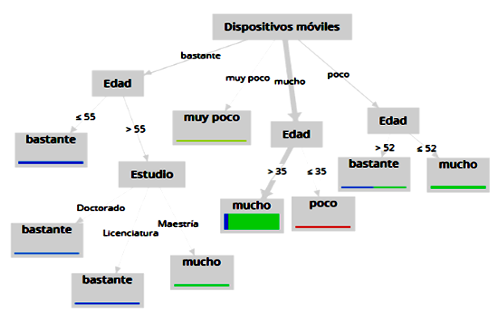
\includegraphics[width=0.7\textwidth]{37074-pag3.png}
 \caption{MP1 sobre los dispositivos móviles.}
 \label{fig3}
 \source{Elaboración propia.}
\end{figure}

En este modelo predictivo, la edad del educador determina 8 condiciones sobre los dispositivos móviles y el uso de la tecnología para la labor docente. Por ejemplo, si el  maestro considera que los dispositivos móviles facilitan mucho la creación de nuevas actividades escolares durante la pandemia COVID-19 y tiene una edad > 35 años, entonces la tecnología favorece mucho la labor docente.

Incluso, el grado de estudio identifica 3 condiciones en el MP1. Por ejemplo, si el  maestro considera que los dispositivos móviles facilitan bastante la creación de nuevas actividades escolares durante la pandemia COVID-19, tiene una edad > 55 años y posee el grado de estudio Maestría, entonces la tecnología favorece mucho la labor docente.

Los resultados del aprendizaje automático com 70\% (0.488, valor\_t = 5.843, valor\_p = 0.000), 60\% (0.558, valor\_t = 6.355, valor\_p = 0.000) y 50\% (0.564, valor\_t = 5.379, valor\_p = 0.000) de entrenamiento indican que la H2 es aceptada (Ver \Cref{tab3}). Por lo tanto, el uso de los dispositivos móviles influye positivamente la participación de los estudiantes durante el proceso de enseñanza-aprendizaje.

La \Cref{fig4} muestra 6 condiciones del MP2 (exactitud de 86.67\%). Por ejemplo, si el maestro considera que los dispositivos móviles facilitan bastante la creación de nuevas actividades escolares durante la pandemia COVID-19 y tiene una edad ≤ 35 años, entonces la tecnología favorece mucho la participación de los estudiantes durante el proceso de enseñanza-aprendizaje.

\begin{figure}[htbp]
 \centering
 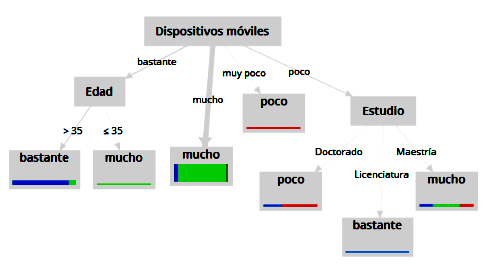
\includegraphics[width=0.7\textwidth]{37074-pag4.png}
 \caption{MP2 sobre los dispositivos móviles.}
 \label{fig4}
 \source{Elaboración propia.}
\end{figure}

En este modelo predictivo, la edad del educador determina 2 condiciones sobre los dispositivos móviles y el uso de la tecnología para la participación de los estudiantes. Por ejemplo, si el maestro considera que los dispositivos móviles facilitan bastante la creación de nuevas actividades escolares durante la pandemia COVID-19 y tiene una edad > 35 años, entonces la tecnología favorece bastante la participación de los estudiantes durante el proceso de enseñanza-aprendizaje.

Incluso, el grado de estudio identifica 3 condiciones en el MP2. Por ejemplo, si el docente considera que los dispositivos móviles facilitan poco la creación de nuevas actividades escolares durante la pandemia COVID-19 y posee el grado de estudio Doctorado, entonces la tecnología favorece poco la participación de los estudiantes durante el proceso de enseñanza-aprendizaje.

Según los maestros de la Universidad Nacional Autónoma de México, el empleo de los dispositivos móviles en las actividades y prácticas educativas favorece la interacción desde cualquier lugar y la comunicación entre los participantes del proceso educativo:

\begin{quote}
“Favorecen la interacción, permiten mantener comunicación constante” (Profesor 2, Maestría, mujer, 39 años).

“Establecer comunicación instantánea con todos” (Profesor 12, Maestría, mujer, 53 años).

“Permiten diversas formas de interacción y comunicación entre los estudiantes” (Profesor 57, Maestría, mujer, 47 años).
\end{quote}

Asimismo, el empleo de los dispositivos móviles mejora el proceso de enseñanza-aprendizaje debido a que estas herramientas tecnológicas permiten el uso de diversas aplicaciones y ofrecen flexibilidad de tiempo y espacio:

\begin{quote}
“Flexibilidad en el manejo de tiempo y espacios” (Profesor 1, Maestría, mujer, 44 años).

“Que se puede acceder a información desde cualquier sitio, se pueden utilizar una diversidad más grande de herramientas digitales para favorecer el aprendizaje, los alumnos pueden aprender a su propio ritmo” (Profesor 21, Maestría, mujer, 37 años).

“Potencian el aprendizaje a partir de recursos multimedia, favorecen el trabajo sincrónico y asincrónico a distancia” (Profesor 32, Licenciatura, mujer, 51 años).
\end{quote}

Algunos beneficios de los dispositivos móviles son el acceso a los contenidos de los cursos, la búsqueda de la información y la distribución de tareas en cualquier momento:

\begin{quote}
“Favorecen la interacción, búsqueda, organización, presentación de información” (Profesor 8, Maestría, mujer, 53 años).

“Puedes acceder fácilmente a la información, realizar tareas, compartir información y comunicarte con los alumnos todo el tiempo en donde quiera que te encuentres” (Profesor 13, Licenciatura, mujer, 44 años).

“Múltiples, la conexión se puede dar en cualquier lugar y las sesiones pueden ser grabadas” (Profesor 45, Licenciatura, mujer, 27 años).
\end{quote}

Incluso, los maestros de la Universidad Nacional Autónoma de México consideran que los dispositivos móviles permiten la organización y creación de nuevos lugares virtuales para el aprendizaje y la enseñanza:

\begin{quote}
“Mejoran las estrategias de enseñanza y aprendizaje, simplifican muchos procesos” (Profesor 5, Maestría, mujer, 41 años).

“Brindan a los profesores y alumnos la posibilidad de contar con más recursos educativos” (Profesor 18, Doctorado, hombre, 55 años).

“Facilita el acceso a recursos, establece una dinámica de comunicación remota, propicia la motivación de los estudiantes, genera nuevos entornos de aprendizaje” (Profesor 46, Maestría, mujer, 50 años).
\end{quote}

De acuerdo con los educadores, los estudiantes tienen la posibilidad de utilizar las plataformas web educativas para consultar los contenidos, entregar las tareas y realizar los foros de discusión en cualquier momento por medio de los dispositivos móviles:

\begin{quote}
“Permiten estar en constante comunicación con los alumnos, hacer consultas, usar plataformas educativas de forma constante, hacer actividades asíncronas” (Profesor 19, Doctorado, hombre, 52 años).

“Permiten acercar la información de manera inmediata, permiten el intercambio de información y materiales, favorecen el trabajo colaborativo, permiten el desarrollo de la actividad” (Profesor 30. Licenciatura, mujer, 56 años).

“Muchos, simplemente la conectividad, la facilidad de poder estar a la distancia en un lugar de manera virtual, la facilidad de obtener información en el momento, compartir información datos documentos, hablar con las personas, tomar fotografías, videos” (Profesor 31, Maestría, mujer, 45 años).
\end{quote}

La \Cref{fig5} muestra la nube de palabras sobre el empleo de dispositivos móviles en el campo educativo donde las palabras con mayor frecuencia son información (n = 22), alumnos (n = 13), comunicación (n = 9), aprendizaje (n = 7), interacción (n = 7), acceso (n = 6),  actividades (n = 6) y estudiantes (n = 6).

\begin{figure}[htbp]
 \centering
 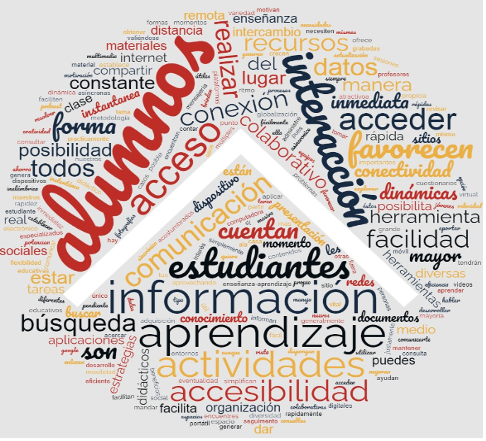
\includegraphics[width=0.7\textwidth]{37074-pag5.png}
 \caption{Nube de palabras sobre los dispositivos móviles.}
 \label{fig5}
 \source{Elaboración propia.}
\end{figure}

\subsection{Juegos web}
Los juegos web facilitan mucho (n = 29, 48.33\%), bastante (n = 15, 25.00\%), poco (n = 8, 13.33\%) y muy poco (n = 8, 13.33\%) la creación de nuevas actividades escolares durante la pandemia COVID-19 (Ver \Cref{tab1}). Los resultados de la técnica aprendizaje automático con 70\% (0.275, valor\_t = 3.264, valor\_p = 0.002), 60\% (0.273, valor\_t = 2.863, valor\_p = 0.007) y 50\% (0.312, valor\_t = 2.920, valor\_p = 0.007) de entrenamiento indican que la H3 es aceptada (Ver \Cref{tab3}). Por lo tanto, el uso de los juegos web influye positivamente la labor docente.

La \Cref{fig6} muestra 8 condiciones del MP3 (exactitud de 88.33\%). Por ejemplo, si el maestro considera que los juegos web facilitan bastante la creación de nuevas actividades escolares durante la pandemia COVID-19 y tienen una edad > 39.5 años, entonces la tecnología favorece bastante la labor docente.

\begin{figure}[htbp]
 \centering
 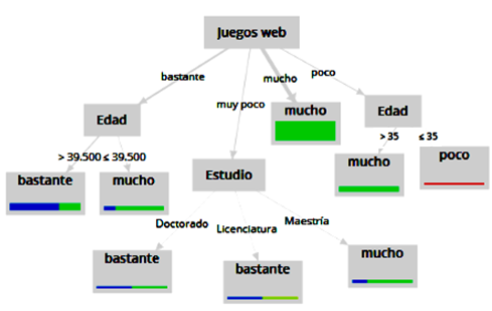
\includegraphics[width=0.7\textwidth]{37074-pag6.png}
 \caption{MP3 sobre los juegos web.}
 \label{fig6}
 \source{Elaboración propia.}
\end{figure}

En este modelo predictivo, la edad del educador determina 4 condiciones sobre los juegos web y el uso de la tecnología para la labor docente. Por ejemplo, si el maestro considera que los juegos web facilitan poco la creación de nuevas actividades escolares durante la pandemia COVID-19 y tienen una edad ≤ 35 años, entonces la tecnología favorece poco la labor docente.

Incluso, el grado de estudio identifica 3 condiciones en el MP3. Por ejemplo, si el docente considera que los juegos web facilitan muy poco la creación de nuevas actividades escolares durante la pandemia COVID-19 y posee el grado de estudio Doctorado, entonces la tecnología favorece bastante la labor docente.

Los resultados de la técnica aprendizaje automático con 70\% (0.262, valor\_t = 3.216, valor\_p = 0.003), 60\% (0.252, valor\_t = 2.754, valor\_p = 0.009) y 50\% (0.253, valor\_t = 2.416, valor\_p = 0.022) de entrenamiento indican que la H4 es aceptada (Ver \Cref{tab4}). Por lo tanto, el uso de los juegos web influye positivamente la participación de los estudiantes durante el proceso de enseñanza-aprendizaje.

La \Cref{fig7} presenta 9 condiciones del MP4 con la exactitud de 78.33\%. Por ejemplo, si el docente considera que los juegos web facilitan mucho la creación de nuevas actividades escolares durante la pandemia COVID-19 y tienen una edad ≤ 56.5 años, entonces la tecnología favorece mucho la participación de los estudiantes durante el proceso de enseñanza-aprendizaje.

\begin{figure}[htbp]
 \centering
 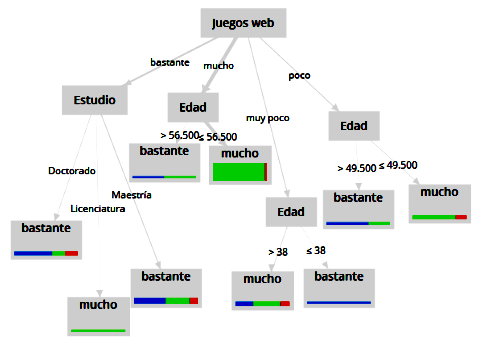
\includegraphics[width=0.7\textwidth]{37074-pag7.png}
 \caption{MP4 sobre el uso de los juegos web.}
 \label{fig7}
 \source{Elaboración propia.}
\end{figure}

En este modelo predictivo, la edad del educador determina 6 condiciones sobre los juegos web y el uso de la tecnología para la participación de los estudiantes. Por ejemplo, si el docente considera que los juegos web facilitan mucho la creación de nuevas actividades escolares durante la pandemia COVID-19 y tienen una edad > 56.5 años, entonces la tecnología favorece bastante la participación de los estudiantes durante el proceso de enseñanza-aprendizaje.

Incluso, el grado de estudio identifica 3 condiciones en el MP4. Por ejemplo, si el docente considera que los juegos web facilitan bastante la creación de nuevas actividades escolares durante la pandemia COVID-19 y posee el grado de estudio Doctorado, entonces la tecnología favorece bastante la participación de los estudiantes durante el proceso de enseñanza-aprendizaje.

Actualmente, los docentes buscan nuevas formas y medios para mejorar e innovar el proceso de enseñanza-aprendizaje. Por ejemplo, los juegos web permiten actualizar las actividades escolares:

\begin{quote}
“Dinamiza la clase” (Profesor 1, Maestría, mujer, 44 años).
“Permiten sesiones más activas e inclusivas” (Profesor 26, Doctorado, mujer, 41 años).

“Son reforzadores de la conducta, por lo tanto, los juegos digitales web como Kahoot son benéficos para cierto tipo de educación, en particular para la educación basada en competencias con criterios cerrados de evaluación, pues permite medir puntualmente las capacidades de los alumnos en habilidades definidas” (Profesor 57, Maestría, mujer, 47 años).
\end{quote}

Según los maestros de la Universidad Nacional Autónoma de México, el empleo de los juegos web incrementa el interés de los alumnos durante la ejecución del proceso de enseñanza-aprendizaje:

\begin{quote}
“Promueven interés en los estudiantes, generan cierta novedad en las acciones y propuestas de aprendizaje” (Profesor 8, Maestría, mujer, 53 años).

“Creación de diversas actividades que pueden ser interesantes para los estudiantes” (Profesor 11, Maestría, hombre, 59 años).

“Promueven un ambiente de aprendizaje lúdico y creativo. Mantienen el interés y la motivación de los alumnos” (Profesor 33, Maestría, mujer, 48 años).
\end{quote}

Incluso, los juegos web permiten la creación de nuevos espacios virtuales donde el estudiante adquiere el rol principal durante la realización del proceso educativo:

\begin{quote}
“Los alumnos corroboran lo aprendido de una manera más amigable, es decir, no se sienten evaluados al momento de utilizar este tipo de actividades, razón por la cual identifican con facilidad sus áreas de oportunidad en un tema específico” (Profesor 15, Maestría, mujer, 36 años).

“Activan el aprendizaje de los estudiantes y permiten al profesor ver si el alumno está aprendiendo” (Profesor 19, Doctorado, mujer, 52 años).

“Los estudiantes son más activos y despierta el interés por competir” (Profesor 38, Maestría, mujer, 47 años).
\end{quote}

Otros beneficios sobre el empleo de los juegos web en el proceso de enseñanza-aprendizaje son la interacción entre los alumnos y el incremento de la motivación :

\begin{quote}
“Facilitan la interacción con los alumnos” (Profesor 5, Maestría, mujer, 41 años).

“Incremento de la motivación en los alumnos, aprender jugando, repaso de temas de forma no tediosa y la autoevaluación” (Profesor 58, Doctorado, mujer 52 años).

“Ofrecen una interacción más dinámica entre alumnos y profesores” (Profesor 34, Licenciatura, mujer, 48 años).
\end{quote}

La \Cref{fig8} presenta la nube de palabras sobre el uso de los juegos web en el campo educativo donde las palabras con mayor frecuencia son alumnos (n = 14), aprendizaje (n = 14), interés (n = 6), evaluación (n = 4), juegos (n = 4), lúdico (n = 4), actividades (n = 3), divertida (n = 3), gamificación (n = 3) y habilidades (n = 3).

\begin{figure}[htbp]
 \centering
 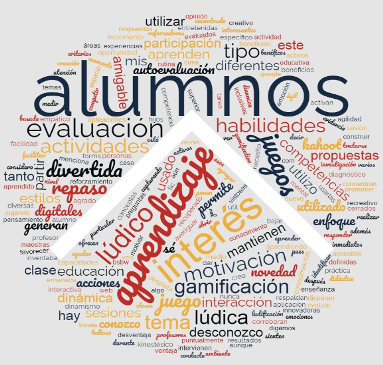
\includegraphics[width=0.7\textwidth]{37074-pag8.png}
 \caption{Nube de palabras sobre los juegos web.}
 \label{fig8}
 \source{Elaboración propia.}
\end{figure}

\section{Discusión}
Varios autores \cite{bawaaneh2021, karatas2021, maphosa2021} mencionan que las herramientas tecnológicas permiten la organización de nuevas actividades educativas y facilitan la participación de los alumnos en cualquier momento y lugar. El 78.33\% de los docentes (n = 47) consideran que la tecnología favorece mucho la labor docente. Asimismo, la tecnología favorece bastante (n = 11, 18.33\%) la labor docente. Por lo tanto, la mayoría de los docentes (96.66\%) tiene una opinión favorable sobre este aspecto.

El 68.33\% de los educadores (n = 41) considera que la tecnología favorece mucho la participación de los estudiantes durante el proceso de enseñanza-aprendizaje. También, la tecnología favorece bastante (n = 14, 23.33\%) la participación. Por lo tanto, la mayoría de los maestros (91.66\%) tiene una opinión favorable sobre este aspecto.

\subsection{Dispositivos móviles}
Los dispositivos móviles permiten la comunicación entre los alumnos durante el proceso de educativo, la planeación de creativas actividades y la interacción entre los docentes y estudiantes desde cualquier lugar \cite{gezgin2018, li2019, padmo2019}. De hecho, los maestros de la Universidad Nacional Autónoma de México consideran que los beneficios de los dispositivos móviles son el acceso a los contenidos de los cursos, la búsqueda de la información y la distribución de tareas en cualquier momento.

El 68.33\% de los maestros (n = 41) consideran que los dispositivos móviles facilitan mucho la creación de nuevas actividades escolares durante la pandemia COVID-19. Asimismo, los dispositivos móviles facilitan bastante (n = 10, 16.67\%) la creación de nuevas actividades escolares durante la pandemia COVID-19. Por consiguiente, la mayoría de los maestros (85.00\%) tiene una opinión favorable sobre el empleo de esta herramienta tecnológica.

Similar a \textcite{li2019}, el uso de los dispositivos móviles transformó la planeación de los cursos y mejoró la interacción durante el proceso educativo. De acuerdo con los participantes de este estudio, el empleo de los dispositivos móviles en las actividades y prácticas educativas favorece la interacción desde cualquier lugar y la comunicación entre los participantes del proceso educativo.

La ciencia de datos establece 9 condiciones del MP1 con una exactitud superior al 93.00\%. En este modelo predictivo, el grado de estudio y la edad de los docentes determinan la relación entre los dispositivos móviles y la labor docente.

Como lo mencionan \textcite{padmo2019}, la incorporación de los dispositivos móviles como los teléfonos inteligentes en el campo educativo permite que los alumnos adquieran un rol activo desde cualquier momento y lugar. Según los maestros de la Universidad Nacional Autónoma de México, el empleo de los dispositivos móviles mejora el proceso de enseñanza-aprendizaje debido a que estas herramientas tecnológicas permiten el uso de diversas aplicaciones y ofrecen flexibilidad de tiempo y espacio.

La ciencia de datos establece 6 condiciones del MP2 con una exactitud superior al 86.60\%. En este modelo predictivo, el grado de estudio y la edad de los docentes determinan la relación entre la participación de los estudiantes y la tecnología.  Por último, los participantes de este estudio consideran que los dispositivos móviles permiten la organización y creación de nuevos lugares virtuales para el aprendizaje y la enseñanza.

\subsection{Juegos web}
Varios autores \cite{donald2017, smith2020, ypsilanti2014} mencionan que los docentes utilizan los juegos web para innovar la organización y ejecución del proceso educativo y facilitar la asimilación del conocimiento. De hecho, los maestros de la Universidad Nacional Autónoma de México mencionan que buscan nuevas formas y medios tecnológicos como los juegos web para mejorar el proceso de enseñanza-aprendizaje y actualizar las actividades escolares.

El 48.33\% de los maestros (n = 29) piensan que los juegos web facilitan mucho la creación de nuevas actividades escolares durante la pandemia COVID-19. Incluso, los juegos web facilitan bastante (n = 15, 25.00\%) la creación de nuevas actividades escolares durante la pandemia COVID-19. Por lo tanto, la mayoría de los maestros (73.33\%) tienen una opinión favorable sobre esta herramienta tecnológica.

Similar a \textcite{de_la_pena_esteban2020}, los juegos web permiten organizar y realizar creativas actividades dentro y fuera del salón de clases. De acuerdo con los participantes de este estudio, el empleo de los juegos web incrementa el interés de los alumnos durante la ejecución del proceso de enseñanza-aprendizaje.
La ciencia de datos presenta 8 condiciones del MP3 con una exactitud superior al 88.00\%. En este modelo predictivo, el grado de estudio y la edad de los docentes determinan la relación entre los juegos web y la labor docente.

Este estudio comparte las ideas de \textcite{donald2017} sobre el empleo de los juegos web en el campo educativo para facilitar la participación y el rol activo de los alumnos. Según los maestros de la Universidad Nacional Autónoma de México, los juegos web permiten la creación de nuevos espacios virtuales donde el estudiante adquiere el rol principal durante la realización del proceso educativo.

La ciencia de datos presenta 9 condiciones del MP4 con una exactitud superior al 78.30\%. En este modelo predictivo, el grado de estudio y la edad de los docentes determinan la relación entre los juegos web y la participación de los alumnos. Por último, los participantes de este estudio consideran que los beneficios sobre el empleo de los juegos web en el proceso de enseñanza-aprendizaje son la interacción entre los alumnos y el incremento de la motivación.

\section{Conclusión}
La pandemia COVID-19 ha provocado que las universidades busquen nuevas alternativas tecnológicas para facilitar el proceso de enseñanza-aprendizaje desde cualquier lugar y la realización de las actividades educativas en cualquier momento. En particular, los resultados de la técnica aprendizaje automático indican que el uso de los juegos web y dispositivos móviles influyen positivamente la labor docente y participación de los alumnos.

Esta investigación cuantitativa y cualitativa recomienda la incorporación de la tecnología en el campo educativo debido a que los docentes pueden crear nuevos espacios virtuales para la enseñanza y el aprendizaje. En particular, los dispositivos móviles y juegos web tienen un papel fundamental para cubrir y satisfacer las demandas educativas originadas por la pandemia COVID-19.

De acuerdo con los maestros de la Universidad Nacional Autónoma de México, los beneficios de los dispositivos móviles son la comunicación, la interacción desde cualquier lugar, el uso de las aplicaciones, la flexibilidad de tiempo y espacio durante el proceso de enseñanza-aprendizaje, el acceso a los contenidos de los cursos, la búsqueda de la información, la distribución de tareas y la creación de nuevos espacios virtuales educativos. Por otro lado, las ventajas de los juegos web son la actualización de los cursos, la interacción, el incremento del interés y la motivación durante la realización de las actividades escolares, el rol activo de los alumnos y la creación de nuevos espacios virtuales.

Las limitaciones de este estudio son la percepción de los docentes, el tamaño de la muestra, el análisis sobre el empleo de los dispositivos móviles y juegos web en el campo educativo y el uso de las técnicas aprendizaje automático y árbol de decisión. Por lo tanto, las futuras investigaciones pueden analizar la incorporación de estas herramientas tecnológicas en las preparatorias, primarias, secundarias y universidades considerando el punto de vista de alumnos y docentes. Asimismo, el uso de los juegos web y dispositivos móviles puede ser analizado considerando la realización de actividades colaborativas y el aprendizaje a distancia. Por último, la técnica de redes neuronal puede utilizarse para identificar los aspectos que influyen durante el empleo de las herramientas tecnológicas.

En conclusión, las instituciones educativas junto con los maestros están transformando el proceso de enseñanza-aprendizaje por medio de la incorporación de las  TIC en las actividades escolares. En particular, los juegos web y dispositivos móviles  permiten construir nuevos espacios educativos que permiten la labor docente y facilitan la participación de los alumnos.

\section*{Agradecimientos}
Trabajo realizado con el apoyo de los Programas UNAM-DGAPA-PAPIME: El Aula del Futuro de la Escuela Nacional Preparatoria 2 (PE208721), El Aula del Futuro de la Escuela Nacional Preparatoria 6 (PE106221), El Aula del Futuro de la Escuela Nacional Preparatoria 8 (PE308221) y El Aula del Futuro de la Facultad de Artes y Diseño (PE402721).


\printbibliography\label{sec-bib}
% if the text is not in Portuguese, it might be necessary to use the code below instead to print the correct ABNT abbreviations [s.n.], [s.l.]
%\begin{portuguese}
%\printbibliography[title={Bibliography}]
%\end{portuguese}


%full list: conceptualization,datacuration,formalanalysis,funding,investigation,methodology,projadm,resources,software,supervision,validation,visualization,writing,review
\begin{contributors}[sec-contributors]
\authorcontribution{Ricardo-Adán Salas-Rueda}[conceptualization,datacuration,formalanalysis,investigation,methodology,validation,writing,review]
\authorcontribution{Jesús Ramírez-Ortega}[funding,investigation,resources,writing,review]
\authorcontribution{Ana-Libia Eslava-Cervantes}[funding,investigation,resources,validation,writing,review]
\authorcontribution{Ricardo Castañeda-Martínez}[funding,formalanalysis,methodology,resources,writing,review]
\authorcontribution{Gustavo De-La-Cruz-Martínez}[conceptualization,datacuration,investigation,resources,writing,review]

\end{contributors}

\end{document}